\subsection{Editor Extension Mechanisms}\label{sec:extension-mechanisms}

This section will describe the extension mechanisms available for the editors in \cref{sec:editors}.

\subsubsection{VSCode Extension}\label{sec:vscode-extension}

\paragraph*{Description}
\Gls{VSCode} extensions are bundles of javascript code and resources in the \texttt{.vsix} file format.
The extensions use a \texttt{package.json} file as a \emph{manifest}, informing VSCode of the \emph{contribution points} used. 
The manifest also indicates \texttt{activation events}, which is \textit{when} an extension will be loaded (they are deactivated by default).~\cite{microsoftExtensionAnatomy2020}
The contribution points can be commands, configuration options, programming language support, debuggers, custom editors etc..~\cite{microsoftContributionPoints2020}
An extension can also contribute views to the VSCode user interface, called the \emph{workbench}, shown in \cref{fig:vscode-workbench-extension}.~\cite{microsoftExtendingWorkbench2020}
The extensions have a main entry point which is called by VSCode in a separate \gls{Nodejs} process called the \emph{Extension host}.~\cite{microsoftExtensionHost2020}
This process isolation improves the stability of VSCode in the case of crashes and hangs in an extension's code.\cite{microsoftExtensionsCapabilitiesOverview2020}

\begin{figure}[htbp]
  \centering
  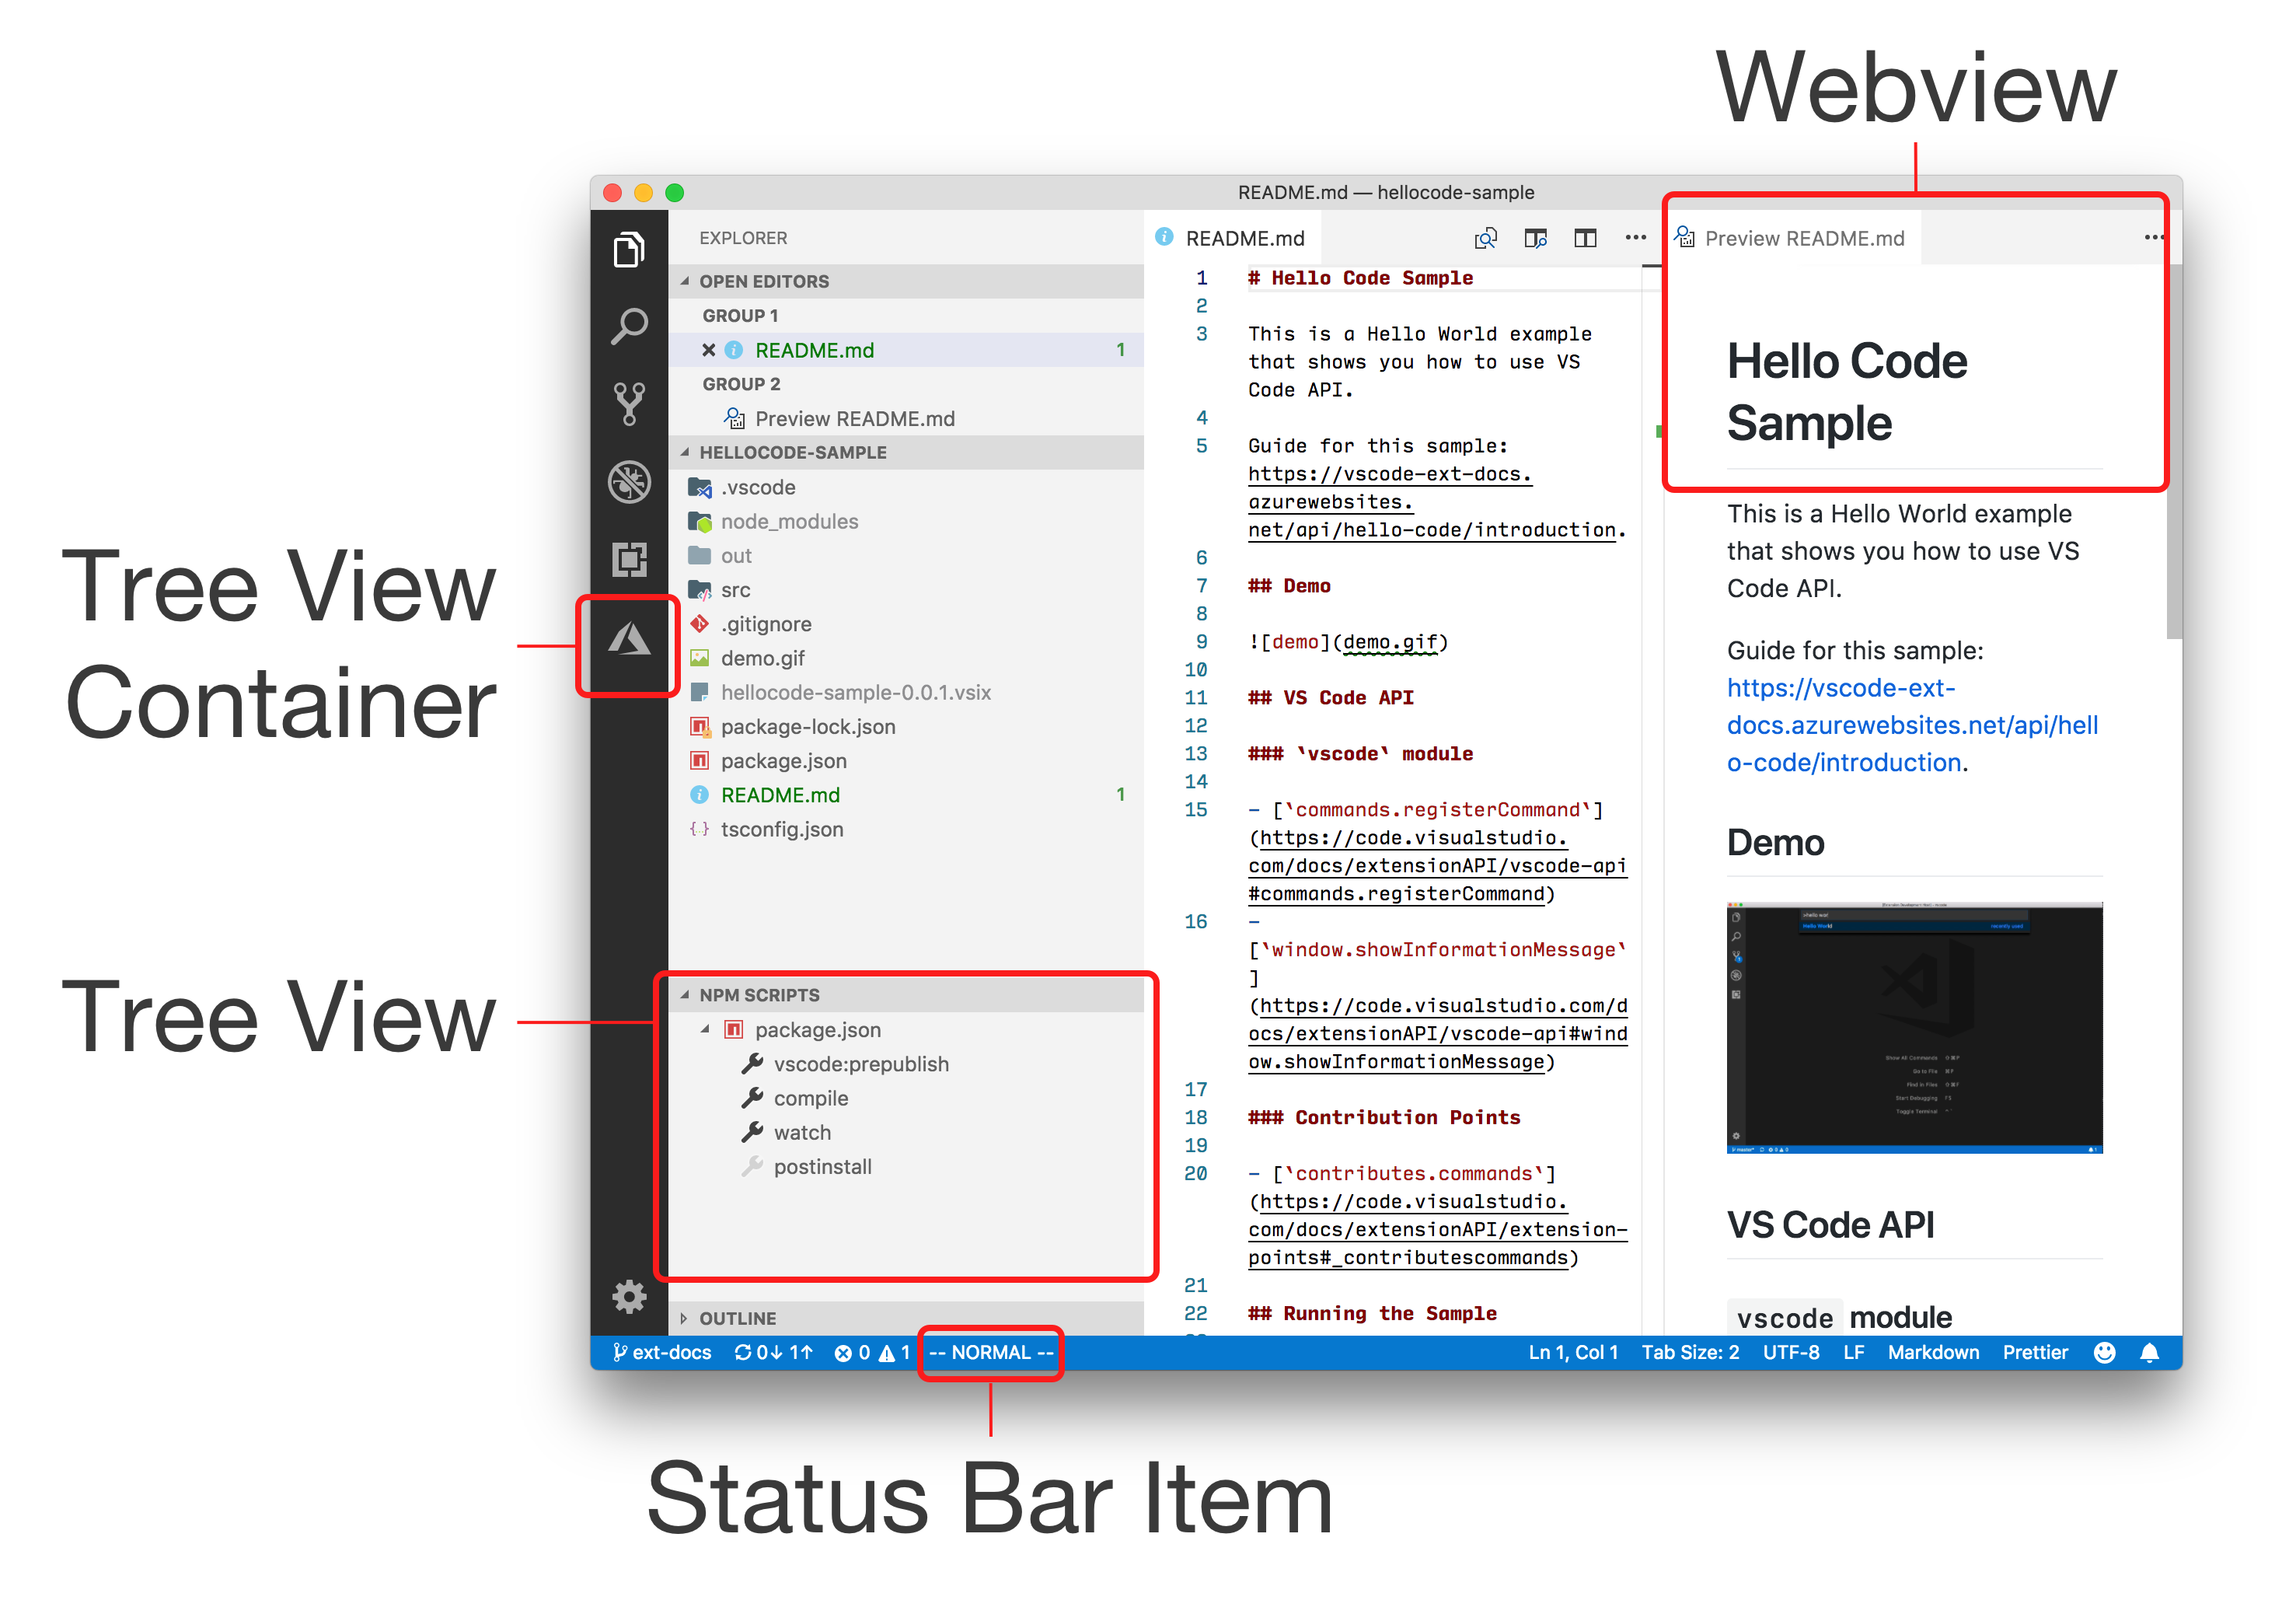
\includegraphics[width=.5\textwidth]{figures/vscode-workbench-contribution.png}
  \caption[VSCode Workbench Extension]{VSCode extensions can extend the different parts of the \emph{workbench}.~\cite{microsoftExtendingWorkbench2020}}\label{fig:vscode-workbench-extension}
\end{figure}

\paragraph*{Restrictions}
Extensions are not allowed to alter the VSCode user interface directly.~\cite{microsoftExtensionsCapabilitiesOverview2020}
All changes must be done via the provided \acrshortpl{API}.
If one wants to create custom HTML elements, the \emph{WebView} \acrshort{API} should be used.
This allows displaying HTML and running javascript.
However, this WebView is also limited: it must communicate with VSCode using \gls{JSON} messages, and relies on VSCode to save its state by handing sending it over.~\cite{microsoftWebviewAPI2020}


%TODO: Write
% Who can use it
% How is it structured?
% What can it do?
% How is it distributed?

\subsubsection{Theia Plugin}\label{sec:theia-plugin}

\paragraph*{Description} \Gls{Theia} \emph{plugins} are exactly the same as VSCode extensions in \cref{sec:vscode-extension}.
A Theia Plugin does not need to separate frontend and backend code.
The VSCode \acrshortpl{API} are transparently separated between the frontend and backend using \gls{JSON-RPC}.~\cite{paulmarechalTheiaPluginImplementation2020}
The support for VSCode extensions was added to Theia so \gls{Che} (which uses Theia) could allow users to install extensions without impacting the stability of the \acrshort{IDE}.~\cite{helmingEclipseTheiaExtensions2019}
A \emph{Theia Extension} could crash and bring down the entire editor, in contrast to a \emph{Theia Plugin} (VSCode extension) which would only display a warning.
Because of licensing issues\footnote{Only Microsoft products can use the marketplace.~\cite{svenefftingeOpenVSX2020}} with Microsoft and its VSCode extension marketplace, all Theia Plugins are hosted on a independent marketplace called \emph{OpenVSX}\footnote{\href{https://open-vsx.org}{https://open-vsx.org}} instead.~\cite{svenefftingeOpenVSX2020}

\paragraph*{Creating a Theia Plugin}
A developer can follow the same tutorials that VSCode Extensions provide, and use the same \acrshortpl{API}.
There is no need to do anything special for Theia to run a VSCode Extension.
However, only a subset of the \acrshortpl{API} are \emph{implemented} yet in Theia.
This is because of time constraints, not policy; more \acrshortpl{API} are supported as developers find time.

\paragraph*{Supported VSCode APIs}
A list of supported \acrshortpl{API} can be found at \href{https://che-incubator.github.io/vscode-theia-comparator/status.html}{https://che-incubator.github.io/vscode-theia-comparator/status.html}.
Most notably for this thesis, is that the \texttt{registerCustomEditorProvider}, \texttt{CustomEditorProvider} and \texttt{createWebviewPanel}\footnote{However, this merge says Theia should support it \href{https://github.com/eclipse-theia/theia/pull/3484}{https://github.com/eclipse-theia/theia/pull/3484}.} are not supported yet.
(Progress for Custom editors can be followed in \href{https://github.com/eclipse-theia/theia/issues/6636}{https://github.com/eclipse-theia/theia/issues/6636}).

\paragraph*{Installing a Theia Plugin}
Either search for the plugin inside the plugin browser provided by \gls{Theia},
or drag-and-drop a \texttt{.vsix} file into the extension browser.
Theia will only search for plugins on OpenVSX, not the Visual Studio Marketplace.

% Who can use it
% How is it structured?
% What can it do?
% How is it distributed?


\subsubsection{Theia Extension}\label{sec:theia-extension}

\paragraph*{Description}
\Gls{Theia} Extensions are the building blocks of Theia.
They are loaded at launch time, not run time.
Dependency injection is used to discover and load extensions.
Extensions were the original mechanism added to Theia for customizing its behavior.
They are allowed full access to Theia, and can do anything\footnote{Within the scope of browsers and \gls{Nodejs}.}.~\cite{helmingEclipseTheiaExtensions2019,helmingEclipseTheiaIDE2019a}
All the main features of Theia are provided using Theia Extensions.

\paragraph*{Installing an extension}
To install a Theia Extension, a developer has to compile Theia itself.
The extension must be available as a package, e.g.\ on \gls{NPM} or as a local folder, and added to the \texttt{package.json} as a dependency.~\cite{helmingHowAddExtensions2019}
For an \gls{NPM} package, the extension's \texttt{package.json} should contain \texttt{``theia-extension''} in the \texttt{keywords}.~\cite{typefoxAuthoringTheiaExtensions}

% Who can use it
% How is it structured?
% What can it do?
% How is it distributed?

% Eclipse plugin? Probably not